\documentclass{article}
\usepackage{amsmath, amssymb, amsthm, amsfonts}
\usepackage{fullpage}
\usepackage{graphicx}

\newtheorem{theorem}{Theorem}
\newtheorem{lemma}{Lemma}
\newtheorem{corollary}{Corollary}
\newtheorem{definition}{Definition}
\newtheorem{proposition}{Proposition}
\newtheorem{procedure}{Procedure}
\newtheorem{construction}{Construction}
\newtheorem{example}{Example}
\newtheorem{remark}{Remark}
\newtheorem{claim}{Claim}

\newcommand{\Rea}{{\mathbb R}}
\newcommand{\Int}{{\mathbb Z}}
\newcommand{\Rat}{{\mathbb Q}}
\newcommand{\Cmp}{{\mathbb C}}
\newcommand{\Nat}{{\mathbb N}}

\setlength{\oddsidemargin}{.25in}
\setlength{\evensidemargin}{.25in}
\setlength{\textwidth}{6.25in}
\setlength{\topmargin}{-0.0in}
\setlength{\textheight}{8.9in}

\renewenvironment{proof}{\noindent{\bf Proof:} \hspace*{1mm}}{
	\hspace*{\fill} $\Box$ }
\newenvironment{proof_of}[1]{\noindent {\bf Proof of #1:}
	\hspace*{1mm}}{\hspace*{\fill} $\Box$ }
\newenvironment{proof_claim}{\begin{quotation} \noindent}{
	\hspace*{\fill} $\diamond$ \end{quotation}}

\newcommand{\handout}[6]{
   \renewcommand{\thepage}{#1-\arabic{page}}
   \noindent
   \begin{center}
   \framebox{
      \vbox{
    \hbox to 5.78in { {\bf #2} \hfill #3 }
       \vspace{4mm}
       \hbox to 5.78in { {\Large \hfill #4  \hfill} }
       \vspace{2mm}
       \hbox to 5.78in { {\it #5 \hfill #6} }
      }
   }
   \end{center}
   \vspace*{4mm}
   \medskip {\large \noindent {\bf NOTE: } \bf The content of these notes has not been formally reviewed by the lecturer. It is recommended that they are read critically.}
}

\newcommand{\lecture}[3]{\handout{#1}{Ubinet, Distributed Optimization and Games 2016-2017}{#2}{Lecture #1}{Lecturer: Giovanni Neglia}{Scribe: #3}}



\usepackage[super]{nth} 
\begin{document}

%header --- replace with appropriate values
\lecture{6}{January 25, 2017}{Dmytro Rubanov}





%start notes here
\section{Introduction}

In this lecture we wil continue to study applications of the Game Theory to distributed optimization problems.

In the section \ref{sec:auctions} we will find a Nash equilibrium strategy for a \nth{1} price auction. We will compare expected seller's revenue in the cases of a \nth{1} price and a \nth{2} price auctions.

In the section \ref{sec:m-markets} we will study a \textit{matching market} that is a problem of assigning several goods to several buyers that have some preferences. We will see how this problem can be solved by introducing \textit{market cleaning prices} that buyers must pay to get a good.

In the section \ref{sec:ads} we will study two approaches for the advertisement pricing: \textit{Vickrey-Clarke-Groves} (\textit{VCG}) mechanism and \textit{Generalized Second Price Auction} (\textit{GSP}). Both of them are generalizations of a \nth{2} price auction for one good. We will see if they encourage buyers to bid truthfully, i. e. set bids equal to their values for a click. We will also compare them in terms of the seller's revenue.

\section{Auctions}\label{sec:auctions}

In the previous lecture we started studying auctions. Now we quickly recap what we have already learned about them.

Let us consider the following problem: there exists a good and a finite set of potential consumers $\{1,..,N\}$, each of them has his ows internal value $v_i$ assigned to the good. The goal is to assing the good to one of the potential consumers in a way that maximizes the total utility. We introduce a set of binary variables $\{x_i\}_{i=1}^N$ with the folowwing meaning:

\begin{equation}
\begin{aligned}
& x_i = 
	\begin{cases}
	1 \hfill & \text{if the good is assigned to the consumer } i\\
	0 \hfill & \text{otherwise}
	\end{cases}
\end{aligned}
\end{equation}
 The problem can be modeled as follows:

\begin{equation}\label{eq:1}
\begin{aligned}
& \underset{\mathbf{x}}{\text{maximize}} 
	& & \sum_{i=1}^N x_i v_i \\
& \text{subject to}
	& & \sum_{i=1}^N x_i = 1 \\
	& & & x_i \in \{0, 1\}
	& & i = 1,..,N
\end{aligned}
\end{equation}

However, each potential consumer $i$ knows only its own value $v_i$ and there is no central authority that knows all the values $\{v_i\}_{i=1}^N$. If potential customers communicate, they may have incentive to lie about their values.

To solve the problem we introduce money. The seller organizes a closed auction, where each potential consumer (bidder, player) chooses a bid $b_i$ and sends it to the seller. The bid $b_i$ is determined by the value $v_i$ and by the strategy of the player $i$. The seller gives the good to the player $i$ with the highest bid $b_i$ and charges it amount $p$ that is determined by the type of the auction. 

Each players chooses his bids to maximize his utility. The utility $U_i$ of the player $i$ is given by the following expression:

\begin{equation}\label{eq:2}
\begin{aligned}
& U_i = 
	\begin{cases}
	v_i - p \hfill & \text{if } x_i = 1\\
	0 \hfill & \text{if } x_i = 0
	\end{cases}
\end{aligned}
\end{equation}

The seller's utility is the price of the good $U_s = p$. One can see that the total utility determined by the equation (\ref{eq:1}) is equal to the sum of the bidders' utilities (\ref{eq:2}) plus the seller's utility.

From now on we will use a notation $\hat i$ to refer to the player with the $i$-th highest bid. $b_{\hat1} > b_{\hat2} > ... > b_{\hat N}$.

\subsection{\nth{2} price auction}

In the case of a \nth{2} price auction the good is given to the player with the highest bid $b_{\hat1}$ and the winner is charged the amount of the second highest bid $p = b_{\hat2}$.

In the previous lecture we have proved that there exists a strictly dominant strategy that is truthful, i. e. each player should set $b_i = v_i$. 

Let us now find the expected sellers revenue. \textbf{We assume that the values $\{v_i\}_{i=1}^N$ are independently uniformly distributed over the interval $[0, 1]$}. In this case the expectation of the $i$-th highest value is:

\begin{equation}
\mathbb{E}(v_{\hat i}) = \frac{N+1-i}{N+1}
\end{equation}

Since the seller's revenue is $U_s = p = b_{\hat2} = v_{\hat2}$,

\begin{equation}\label{eq:sel-rev-2nd-price}
\mathbb{E}(U_s) = \frac{N-1}{N+1}
\end{equation}

The result is supported by the fact that the seller's revenue should converge to its maximum value 1 with increase of the number of players.

\subsection{\nth{1} price auction}

Now we consider a \nth{1} price auction, where the player with the highest big $b_{\hat1}$ gets the good and pays the amount of his bid $p = b_{\hat1}$.

In this case, being thruthful is not a dominant strategy anymore. To study this type of auctions we make the following assumption: \textbf{for each player the values of other players are independently uniformly distributed over the interval $[0, 1]$}.

Since all the players are equivalent, they should use the same strategy. A strategy is a mapping $s()$ such that $b_i = s(v_i)$ for all $i\in\{1,..,N\}$. This strategy has the following properties:

\begin{itemize}
	\item $s()$ is strictly increasing because the more we value the product the more we are ready to pay for it;
	\item if $v > 0$ then $s(v) < v$ because the player's utility is positive only if he pays less than the value;
	\item $s(0) = 0$ because a player will not buy a good that has no value;
	\item we also suppose $s()$ to be continuous and differentiable because there are no special points where these properties may be violated.
\end{itemize}

We investigate if there exists such a strategy $s()$ that leads to a Nash equilibrium.

Since $s()$ is increasing, the winner of the auction is the player with the highest value $v_i$. The probability that the player $i$ with the value $v_i$ wins is the follows:

\begin{equation}
	\mathbb{P}(x_i = 1) = \mathbb{P}\left(b_i = \underset{j \in \{1,.,N\}}{\text{max}} b_j \right) = \mathbb{P}\left(v_i = \underset{j \in \{1,.,N\}}{\text{max}} v_j \right) = \prod_{\substack{j = 1 \\ j \neq i}}^N \mathbb{P}(v_j < v_i) = v_i^{N-1}
\end{equation} 

The expected utility off the player $i$ if all other players play $s()$:

\begin{equation}\label{eq:s-utility}
\begin{aligned}
	& \mathbb{E}\left(U_i(s(v_1),..,s(v_i),..,s(v_n))\right) = \mathbb{P}(x_i = 1) \mathbb{E}(U_i \mid x_i = 1) + \mathbb{P}(x_i = 0) \mathbb{E}(U_i \mid x_i = 0) = \\ 
	& = v_i^{N-1} (v_i-b_i) + \left(1 - v_i^{N-1}\right) \cdot 0 = v_i^{N-1} (v_i-s(v_i))
\end{aligned}
\end{equation}

Now let the player $i$ use another strategy $t()$. If everyone using $s()$ is a NE, than using $t()$ instead of $s()$ would be a worse choice for the player $i$.

\begin{equation}\label{eq:ne-condition}
\mathbb{E}\left(U_i(s(v_1),..,s(v_i),..,s(v_n))\right) \ge \mathbb{E}\left(U_i(s(v_1),..,s(v_{i-1}),t(v_i),s(v_{i+1}),..,s(v_n))\right)
\end{equation}

Unfortunately, it is extrimely difficult to check all possible strategies $t()$. However, due to the \textbf{revelation principle}, changing the strategy from to $t()$ is equivalent to providing the strategy $s()$ with a value $v$ such that

\begin{equation}
b_i = t(v_i) = s(v)
\end{equation}

Utility of the player $i$ is

\begin{equation}\label{eq:t-utility}
\begin{aligned}
	& \mathbb{E}\left(U_i(s(v_1),..,s(v_{i-1}), t(v_i),s(v_{i+1}),..,s(v_n))\right) = \\
	& = \mathbb{E}\left(U_i(s(v_1),..,s(v_{i-1}), s(v),s(v_{i+1}),..,s(v_n))\right) = v^{N-1}(v_i-s(v))
\end{aligned}
\end{equation}

From equations (\ref{eq:s-utility}), (\ref{eq:ne-condition}) and (\ref{eq:t-utility}) we get the following condition if everyone using $s()$ is a NE:

\begin{equation}
\begin{aligned}
	\forall v \in [0, 1] & & v_i^{N-1}(v_i-s(v_i)) \ge v^{N-1}(v_i-s(v))
\end{aligned}
\end{equation}

Let us consider a function $f(v)$, such that

\begin{equation}
f(v) = v_i^{N-1}(v_i-s(v_i)) - v^{N-1}(v_i-s(v))
\end{equation}

This function must have a minimum at the point $v = v_i$. Hence, its derivative at this point must to equal to zero.

\begin{equation}
\begin{aligned}
	& f'(v) = -(N-1)v^{N-2}(v_i-s(v)) + v^{N-1}s'(v) \\
	& f'(v)\big|_{v=v_i} = -(N-1)v_i^{N-2}(v_i-s(v_i)) + v_i^{N-1}s'(v_i) = 0                    \\
	& s'(v_i) = (N-1)\left(1 - \frac{s(v_i)}{v_i}\right)
\end{aligned}
\end{equation}

The differential equation above must be true for any $v_i \in [0, 1]$. The solution to it, with respect to the initial condition $s(0) = 0$, is the follows:

\begin{equation}
s(v_i) = \frac{N-1}N v_i
\end{equation} 

That means that if every player bids $b_i = (N-1)/N \cdot v_i$ we achieve a NE. We see that each of them should always bid less then his value. Bids converge to values if the number of players increases.

Let us now compute the expectation of the seller's revenue.

\begin{equation}\label{eq:sel-rev-1st-price}
\mathbb{E}(U_s) = \mathbb{E}(p) = \mathbb{E}(b_{\hat1}) = \frac{N-1}N \mathbb{E}(v_{\hat1}) = \frac{N-1}N \frac N{N+1} = \frac{N-1}{N+1}
\end{equation}

One can compare (\ref{eq:sel-rev-2nd-price}) and (\ref{eq:sel-rev-1st-price}) and see that seller's revenues are equivalent in the cases of a \nth{2} price and a \nth{1} price auction. This is a consequence of the general \textbf{revenue equivalence principle}.

\section{Matching markets}\label{sec:m-markets}

Let us now have $M$ goods $N$ buyers. Each buyer assigns a value to each good. We define $v_{ij}$ as the value that buyer $j$ gives to good $i$. Clearly these values can be different. We would like to assign goods to buyers in such a way that maximizes the social utility. This problem can be modeled as a linear program.

\begin{equation}
\begin{aligned}
\text{Let } x_{ij}= 
\begin{cases}
	1 \hfill & \text{ if good \textit{i} is assigned to buyer \textit{j}} \\
	0 \hfill &\text{ otherwise}\\
\end{cases}
\end{aligned}
\end{equation}

The problem can be formulated in the following way:
\begin{equation}
\begin{aligned}
& \underset{X}{\textrm{maximize} }
& & \sum_{i=1}^{N}\sum_{j=1}^{M} x_{ij}v_{ij}\\
& \textrm{subject to } 
	&& \sum_{j=1}^N x_{ij}=1, & & i=1,.., M \\
	&&& \sum_{i=1}^M x_{ij}=1, & & j=1,.., N\\	
	&&& x_{ij} \in \{0,1\},  & & i=1,.., M & &  j=1,.., N \\
\end{aligned}
\end{equation}

The objective function expresses our purpose to maximize the sum of the values that each buyer would have in the assignment. The first set of constraint expresses the fact that each good is assigned to just one buyer. The second set of constraint express the fact that to each buyer is assigned just one good.

As in the previous case we can't ask buyers about the value that they give to each good because they could lie since there is no incentive for them to say the truth. So like in the auction case we need to introduce money in the form of prices.

We can assign a price $p_i$ to each good $i$, and ask the the buyers which good they prefer. Each buyer $j$ by computing $v_{ij}-p_i$ can calculate the utility that he would get if he acquired the good $i$ and will answer with the good (or goods in case they are more than one) that allow him to get the maximum utility. Based on the answers we can build a \textbf{preference graph}.

Let us consider the following example:

\centerline{
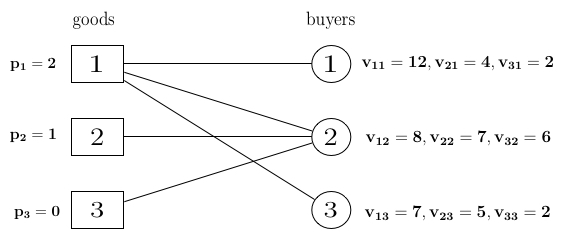
\includegraphics[width=300pt]{img12.jpg}}

In this case buyer 1 would prefer good 1 since his payoffs based on the prices are $(10,3,2)$ and good 1 give him the maximum payoff. For buyer 2 it's equivalent to get good 1, 2 or 3 since his payoff are $(6,6,6)$. Buyer 3 would prefer good 1 since it's the one that gives him the higher payoff, in fact his payoff are $(5,4,2)$.

Given these preferences we draw an arrow between each buyer and his preferred good (or goods). A perfect matching in the graph would be an assignment of goods to buyers. Unfortunately, the graph of our example does not have a perfect matching. What we can try to do is to change the prices. For example, let's increase the price of $p_1$ from 2 to 3. The new preference graph, due to this change, would be different:

\centerline{
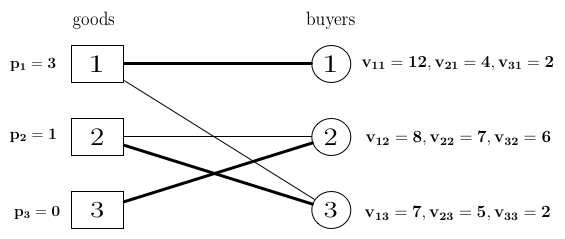
\includegraphics[width=300pt]{img13.jpg}}

In fact now buyer 2 would not prefer anymore good 1 since his payoffs now are $(5,6,6)$ and buyer 3 would prefer not just good 1 but also good 2 since his payoffs now are $(4,4,2)$. Even if the price for good 1 has changed buyer 1 continues to prefer just good 1.

In this graph we can find a perfect matching that in the case of the graph corresponds to the assignment: 

\begin{itemize}
	\item good 1 to buyer 1 
	\item good 2 to buyer 3 
	\item good 3 to buyer 2 
\end{itemize}

The total social utility for this assignment would be:

\begin{equation}
v_{11}+v_{23} +v_{32}=12+5+6=23
\end{equation}

It is optimal is the sense that we can't find any other assignment that would give has a higher social utility.

The prices so determined are called \textbf{Market Clearing Prices}. Market Clearing Prices are those prices that allow to assign all the goods in the market (that means find a perfect matching) and they achieve the maximum total valuation of any assignment of sellers to buyers. Two important properties of the Market Clearing Prices are that they always exist and that they maximize the global payoff for both sellers and buyers. However, we need to know the valuations of the buyers to calculate them.

\section{Approaches for the advertisement pricing}\label{sec:ads}

In this last section we will try to put together the \textit{matching market}, where we know that Market Clearing Prices exist, and \textit{auctions}, where we want to define a mechanism that brings the bidders to reveal the real value that they assign to each good.

The problem for an advertising company like \textit{Google} is to find a matching bewteen advertisements (ads) position and companies. We can assign to each position a value $r_i$ defined as the click rate for an ad in position $i$. This rate is known a priori. Each company has a value $v_i$ defined as the value that company $i$ gives to a click. Knowing this information we would be able to calculate the value of a given position for each company. In fact, the value of $r_i$ click for company $i$ is given by $v_ir_i$.

We would have the following problem:

\centerline{
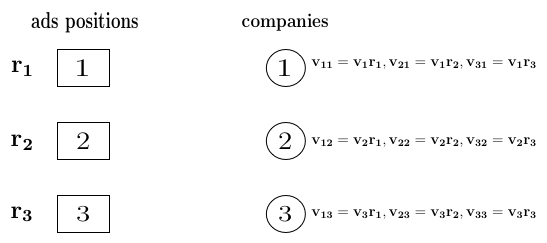
\includegraphics[width=300pt]{img14.jpg}}

As we can see the problem would become the same as the Matching Market that is to find Market Clearing Prices. To do this we need to know the value $v_i$ for each company. What we can do it to set up an auction where companies bid the value for a click $b_i$ and we assign the $N$ ads positions $r_1,...,r_N$ to the companies considering their $b_i$ in non increasing order: the best position is assigned to the company that has bid the most, the second best position is assigned to the company that has bid the second value and so on.

We know that \nth{2} price auction is a truthful mechanism in case of single item auction. We would like to generalize this mechanism for multiple items auction. The first idea could be to use the natural extension of the \nth{2} price auction in which the highest bidder gets the first position and pays the price bid by the second-highest bidder, the second-highest gets the second position and pays the price bid by the third-highest bidder, and so on. This mechanism is called \textbf{Generalized second-price auction} or \textbf{GSP}. Unfortunately GSP is not a truthful mechanism.

\subsection{Vickrey-Clarke-Groves mechanism}\label{subsec:VCG}

The correct way to generalize the \nth{2} price auction that provides us a truthful mechanism is the \textbf{VCG} (Vickrey-Clarke-Groves). In a VCG auction every buyers should pay a price equal to the social value loss for the others buyers. This means that a buyer should pay the difference between what the other players would have got if he were not be there and what they  get if he is there.

Suppose to have an auction for a single item and that the bids are such that $b_{\hat1}>b_{\hat2}>...>b_{\hat N}$; so buyer $\hat1$ would get the item. Let us consider the social utility for the buyers $\hat2,\hat3,..,\hat N$:

\begin{itemize}
	\item if buyer $\hat1$ is not present it would be $v_{\hat2}$ ($b_{\hat2}=v_{\hat2}$ being VCG a truthful mechanism). In this case buyer $\hat2$ would get the item since by hypothesis $b_{\hat2}$ is the second highest bid, the other buyers ($\hat3,..,\hat N$) would have an utility equal to $0$ because of the the fact that they don't get the item. 
	\item if buyer $\hat1$ is present it would be $0$, since buyer $\hat1$ get the item and for all the other, since no one of them get the item, the utility would be $0$ 
\end{itemize}

So for single item auction the winner should play $v_{\hat2}-0=v_{\hat2}$. VCG in the case of single item auction become the \nth{2} price auction. Moreover, $v_2$ is not just the second price but it's also the damage done to the society.

In case of multiple items auction, let $V_{B}^{S}$ be the maximum total valuation over all the possible perfect matchings between the set of sellers S and the set of buyers B. If buyer j gets good i, he should pay the difference between the total valuation that the other people get if j would not be there dividing by them the set of goods ($V_{B-j}^{S}$) and the total valuation that the other people get if j would be there ($V_{B-j}^{S-i}$) dividing by them the set of goods except good i. Under this price mechanism, truth-telling is a dominant strategy.

Let's make an example. There are 3 ads position with a click rate of $10$ for \nth{1} position ($r_1=10$),$5$ for \nth{2} position ($r_2=5$) and $2$ for \nth{3} position ($r_3=2$). Moreover we have 3 companies for which the values of a click is 3 for company 1 ($v_1=3$), 2 for company 2 ($v_2=2$) and 1 for company 3 ($v_3=1$).

These informations are enough to calculate the value that each company gives to each position.

\centerline{
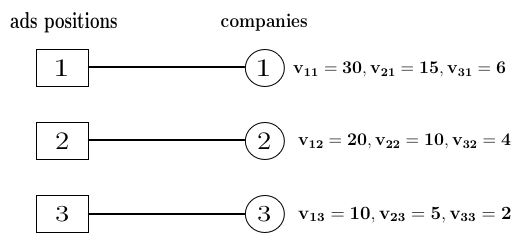
\includegraphics[width=300pt]{img15.jpg}}

Moreover we can see that the maximum weight perfect matching is the one that assign position 1 to company 1, position 2 to company 2 and position 3 to company 3. This assignment gives us a total valuation of $42$ (so $V_{B}^{S}=42$). In fact company 1 gets 30, company 2 gets 10 and company 3 gets 2. 

Now let's calculate how much each company should play according to VCG mechanism.

\paragraph{Company 1} 

In our optimal allocation the total valuation that companies 2 and 3 get if company 1 participate is 12. But if company 1 did not participate we would have the following allocation for companies 2 and 3

\centerline{
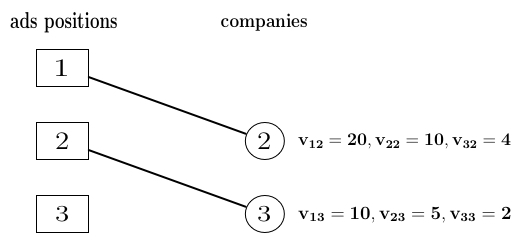
\includegraphics[width=300pt]{case1.jpg}}

So if company 1 did not participate the total valuation that companies 2 and 3 get would be 25. So company 1 should pay $V_{B-1}^{S}-V_{B-1}^{S-1}=25-12=13$

\paragraph{Company 2}

In our optimal allocation the total valuation that companies 1 and 3 get if company 2 participate is 32. But if company 2 did not participate we would have the following allocation for companies 1 and 3

\centerline{
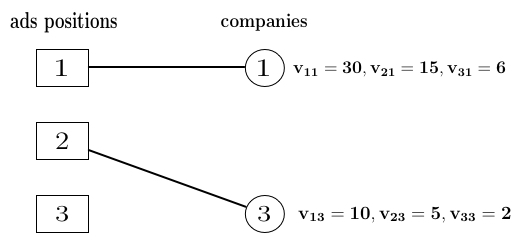
\includegraphics[width=300pt]{case2.jpg}}

So if company 2 did not participate the total valuation that companies 1 and 3 get would be 35. So company 1 should pay $V_{B-2}^{S}-V_{B-2}^{S-2}=35-32=3$

\paragraph{Company 3}

In our optimal allocation the total valuation that companies 1 and 2 get if company 3 participate is 40. But if company 3 did not participate we would have the same allocation for companies 1 and 2

\centerline{
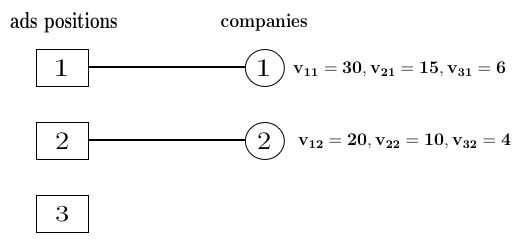
\includegraphics[width=300pt]{case3.jpg}}

So if company 3 did not participate the total valuation that companies 1 and 2 get would be 40. So company 1 should pay $V_{B-3}^{S}-V_{B-3}^{S-3}=40-40=0$

\subsection{Generalized Second Price mechanism}\label{subsec:GSP}

\textit{Google} distributes goods (positions) using \textit{Generalized Second Price} auctions. It collects all the bids $b_{\hat1} > b_{\hat2} > ... > b_{\hat N}$ and assigns to the bidder $\hat i$ the $i$-th best good and charges him $p_{\hat{i}} = b_{\hat{i+1}}$.

Let us consider an example that proves that in $GSP$ being thruthful is not a NE anymore.	Let us consider a case of three ads positions with rates $r_1 = 10$, $r_2 = 4$, $r_3 = 0$ and three companies that give the following values per click $v_1 = 7$, $v_2 = 6$, $v_3 = 1$. If everyone is thrutful, i. e. $b_i = v_i$ for all $i$, the positions are assigned in the following way:

\centerline{
\includegraphics[scale=0.6]{GSP_1.png}}

In this case the first company gets the first position and pays $p_1 = b_2 = 6$ per click. Its utility:

\begin{equation}
U_1(b_1 = 7, b_2 = 6, b_3 = 1) = r_1 (v_1 - p_1) = 10(7-6) = 10
\end{equation}

Let now the first company bid $b_1 = 5$. This changes the distribution:

\centerline{
\includegraphics[scale=0.6]{GSP_2.png}}

The first company gets the second position and pays $p_1 = b_3 = 1$ per click. Its utility is

\begin{equation}
U_1(b_1 = 7, b_2 = 6, b_3 = 1) = r_2 (v_1 - p_1) = 4(7-1) = 24
\end{equation}

Here we see that the first company has incentive to bid less than the value of a click because it would increasy its utility. 

We have seen that the truth is not a NE in the case of \textit{GSP}. However, there always exists at least one another NE. In the example above there are two of them: $(b_1 = 4, b_2 = 4, b_3 = 2)$ and $(b_1 = 3, b_2 = 5, b_3 = 1)$. In the first case the seller's total revenue if 48, in the second it is 34. With \textit{VCG} his revenue would be 44.

\section{Conclusion}

In this lecture we continued studying \textit{auctions} as a game-theoretical mode. Under several assumptions we found a Nash equilibrium  strategy for \nth{1} price auctions. This strategy suggests the players to bid less than they value the good. We also discovered that the expectated seller's revenue is the same for both \nth{1} price and \nth{2} price auctions. It is This is a consequence of the general \textit{revenue equivalence principle}.

We introduced \textit{matching markets} as a problem of making a perfect match between goods and buyers in such a way that maximizes the total utility of both sellers and buyers. If we know the values that buyers assign to goods, this problem can be solved by introducing \textit{marker cleaning prices} that must be paid by users for goods.

We studied two approaches for the advertisements pricing when values that the companies (buyers) give to a click are not known in advance. Both approaches are generalizations of the \nth{2} price auction. With the Vickrey-Clarke-Groves mechanism each company should pay a price equal to the social value loss for the others companies. In this case the gest strategy for each company is to be truthful, i. e. set a bid equal to its value for a click $b_i = v_i$. Another mechanism is a generalized \nth{2} price auction, where a company with $i$-th bid gets $i$-th best position and charged the amount of the next highest bid. We have seen an example that proves that with this mechanism being truthfu may not be a best strategy anymore. The seller's revenue may be both lower or higher compared to the \textit{VCG} mechanism.

%%%%  Bibliography goes here

\begin{thebibliography}{alpha}

\bibitem{Kel14} Frank Kelly and Elena Yudovina,
\newblock Stochastic Networks.
\newblock {\em Cambridge Press}, 2014.

\end{thebibliography}


\end{document}
